\section{Les tableaux à 2 dimensions}
%\leconwithtoc

\subsection{Définition}

\begin{frame}{Définition}
	\begin{itemize}
		\item
		La \textbf{dimension} d’un tableau est le nombre d’indices qu’on utilise
		pour faire référence à un de ses éléments. 
		\item
		Attention de ne pas confondre avec la	taille !
	\end{itemize}
	
	Dans ce qui précède, nous avons introduit les tableaux à une dimension.
	
	Un seul indice suffisait à localiser un de ses éléments. 
	
	De nombreuses	situations nécessitent cependant 
	l’usage de tableaux à deux dimensions.
	
	Ils vous sont déjà familiers par leur présence dans beaucoup de
	situations courantes : calendrier, grille horaire, grille de mots
	croisés, sudoku, jeux se déroulant sur un quadrillage (damier,
	échiquier, scrabble, \dots).
\end{frame}

\subsection{Déclaration}

\begin{frame}{Déclaration}
	Pour déclarer un tableau statique à 2 dimensions, on écrira :

	\cadre{
	\begin{pseudo}
	\Decl nomTableau : \K{tableau} [ligMin à ligMax, colMin à colMax] de TypeElément
	\end{pseudo}
	}
	
	Pour un tableau dynamique, on procédera en deux étapes comme expliqué
	pour les tableaux à une dimension. 
	
	\cadre{
	\begin{pseudo}
	\Decl nomTableau~: \K{tableau} de TypeElément
	\LComment Le code peut déterminer ici les bornes
	\Let nomTableau \Gets \K{nouveau} \K{tableau} [ligneMin à ligneMax, colMin à colMax] de TypeElément
	\end{pseudo}
	}

	où \code{ligneMin}, \code{ligneMax}, 
	\code{colMin} et \code{colMax}sont des
	expressions entières quelconques.
\end{frame}

\begin{frame}{Déclaration}
	On ne se permettra pas en logique de
	combiner les deux types de tableaux, à savoir utiliser la notation
	«~statique~» pour certaines dimensions et «~dynamique~» pour les
	autres.

	Notez qu'un tableau à deux dimensions peut aussi être
	vu comme un tableau à une dimension dont chacun des éléments est
	lui-même un tableau à une dimension.
\end{frame}

\begin{frame}{Exemple} 
	Soit le tableau déclaré ainsi:

	\cadre{
	\begin{pseudo}
	\Decl ntabLettres : \K{tableau}[1 à 4, 1 à 5] de caractères
	\end{pseudo}
	}

	On peut le visualiser à l’aide d’une grille à 4 lignes et 5 colonnes.
\end{frame}

\begin{frame}{Exemple}
	\begin{center}
	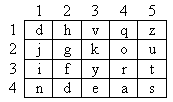
\includegraphics[width=4cm]{image/tab2d-vision-tab2d}
	\end{center}

	Ainsi, la valeur de \code{tabLettres[3,4]} 
	est le caractère ‘r’. 
\end{frame}

\begin{frame}{Exemple}
		La vision «~tableau de tableau~» 
	(ou décomposition en niveaux)
	donnerait :

	\begin{center}
	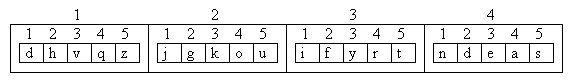
\includegraphics[width=0.9\textwidth]{image/tab2d-vision-tabtab}
	\end{center}

	Dans cette représentation, le tableau \code{tabLettres} est
	d’abord décomposé à un premier niveau en quatre éléments auxquels on
	accède par le premier indice. Ensuite, chaque élément de premier niveau
	est décomposé en cinq éléments de deuxième niveau accessibles par le
	deuxième indice.
\end{frame}

\begin{frame}{Exemple~: Statistiques de vente}
	reprenons l'exemple du stock de 10 produits
	qui a servi d'introduction au chapitre sur les tableaux
	mais, cette fois, pour chaque jour de la semaine.
	
	\begin{small}
	\begin{center}
		\begin{tabular}{*{8}{>{\centering\arraybackslash}m{1.3cm}}}
			~ &
			{article1} &
			{article2} &
			{article3} &
			\dots &
			{article8} &
			{article9} &
			{article10}\\
		\end{tabular}	
		\begin{tabular}{|m{1.3cm}|*{7}{>{\centering\arraybackslash}m{1.3cm}|}}
			\hline
			{lundi} & 
			{cpt[1][1]} &
			{cpt[1][2]} &
			{cpt[1][3]} &
			\dots &
			{cpt[1][8]} &
			{cpt[1][9]} &
			{cpt[1][10]}
			\\\hline
			{mardi} &  
			{cpt[2][1]} &
			{cpt[2][2]} &
			{cpt[2][3]} &
			\dots &
			{cpt[2][8]} &
			{cpt[2][9]} &
			{cpt[2][10]}
			\\\hline
			{mercredi} & 
			{cpt[3][1]} &
			{cpt[3][2]} &
			{cpt[3][3]} &
			\dots &
			{cpt[3][8]} &
			{cpt[3][9]} &
			{cpt[3][10]}
			\\\hline
			{jeudi} & 
			{cpt[4][1]} &
			{cpt[4][2]} &
			{cpt[4][3]} &
			\dots &
			{cpt[4][8]} &
			{cpt[4][9]} &
			{cpt[4][10]}
			\\\hline
			{vendredi} & 
			{cpt[5][1]} &
			{cpt[5][2]} &
			{cpt[5][3]} &
			\dots &
			{cpt[5][8]} &
			{cpt[5][9]} &
			{cpt[5][10]}
			\\\hline
			{samedi} & 
			{cpt[6][1]} &
			{cpt[6][2]} &
			{cpt[6][3]} &
			\dots &
			{cpt[6][8]} &
			{cpt[6][9]} &
			{cpt[6][10]}
			\\\hline
			{dimanche} & 
			{cpt[7][1]} &
			{cpt[7][2]} &
			{cpt[7][3]} &
			\dots &
			{cpt[7][8]} &
			{cpt[7][9]} &
			{cpt[7][10]}
			\\\hline
		\end{tabular}
	\end{center}
	\end{small}
\end{frame}

\begin{frame}{Exemple~: Statistiques de vente}
	\cadre{
	\begin{pseudo}
	\scriptsize{
	\LComment Calcule et affiche la quantité vendue de 10 produits
	\LComment pour chaque jour de la semaine (de 1~: lundi à 7~: dimanche).
	\Module{statistiquesVentesSemaine}{}{}
		\Empty
		\Decl cpt~: \K{tableau} [1 à 7, 1 à 10] d’entiers
		\Decl produit, jour~: entiers
		\Empty
		\Stmt initialiser(cpt)
		\Empty
		\LComment Pour chaque jour de la semaine
		\For{jour \K{de} 1 \K{à} 7}
			\Stmt traiterStock1Jour(cpt, jour)
			\For{produit \K{de} 1 \K{à} 10}
				\Write "quantité vendue de produit ", produit, " ce jour ", jour, "~: ", cpt[jour][i]
			\EndFor
		\EndFor	
	\EndModule
	}
	\end{pseudo}
	}
\end{frame}

\begin{frame}{Exemple~: Statistiques de vente}
	\cadre{
	\begin{pseudo}
	\LComment Ce module initialise le tableau d'entiers à 0
	\Module{initialiser}{entiers\InOut~: \K{tableau} [1 à 7, 1 à 10] d’entiers}{}
		\Decl i, j~: entiers
		\For{i \K{de} 1 \K{à} 7}
			\For{j \K{de} 1 \K{à} 10}
				\Let cpt[i][j] \Gets 0
			\EndFor
		\EndFor
	\EndModule
	\end{pseudo}
	}
\end{frame}

\begin{frame}{Exemple~: Statistiques de vente}
	\cadre{
	\begin{pseudo}
	\scriptsize{
	\LComment Ce module effectue le traitement du stock pour une journée.
	\Module{traiterStock1Jour}{cpt~\InOut: \K{tableau} [1 à 7, 1 à 10] d’entiers, jour~: entier}{}
		\Decl numéroProduit, quantité~: entiers
		\Write "Introduisez le numéro du produit~:"
		\Read numéroProduit
		\Empty
		\While{numéroProduit > 0}
			\Empty
			\Write "Introduisez la quantité vendue~:"
			\Read quantité
			\Empty
			\Let cpt[jour][numéroProduit] \Gets cpt[jour][numéroProduit] + quantité
			\Empty
			\Write "Introduisez le numéro du produit~:"
			\Read numéroProduit
			\Empty
		\EndWhile
	\EndModule
	}
	\end{pseudo}
	}
\end{frame}

\subsection{La troisième dimension (et au-delà)}

\begin{frame}{La troisième dimension (et au-delà)}
	Certaines situations complexes nécessitent l'usage de
	tableaux à 3 voire plus de dimensions.

	Pour déclarer un tableau statique à $k$ dimensions, on écrira :

	\cadre{
	\begin{pseudo}
	\Decl nomTableau : \K{tableau} [ bMin\_1 à bMax\_1, \dots, bMin\_k à bMax\_k] de TypeElément
	\end{pseudo}
	}

	où chaque paire de bornes \code{bMin\_i}~et
	\code{bMax\_i} limite l’indice correspondant 
	à la $i^{ème}$	dimension du tableau.
\end{frame}

\subsection{Parcours d'un tableau à deux dimensions}

\begin{frame}{Parcours d'un tableau à deux dimensions}
	envisageons le parcours des tableaux à deux dimensions 
(n lignes et m colonnes).

Déclaration d'un tableau statique~:

\cadre{
\begin{pseudo}
	\Decl tab~: tableau [1 à n, 1 à m] de T
\end{pseudo}
}

Déclaration d'un tableau dynamique~:

\cadre{
	\begin{pseudo}
	\Decl tab~: \K{tableau} de T
	\Let tab \Gets \K{nouveau} \K{tableau} [1 à n, 1 à m] de T
	\end{pseudo}
}
\end{frame}

\begin{frame}{Parcours d'un tableau à deux dimensions}	
	Commençons par des cas plus simples 
	où on ne parcourt qu'une seule des dimensions 
	puis attaquons le cas général.
\end{frame}

\begin{frame}{Parcours d'un tableau à deux dimensions~: parcours d'une dimension}	
	On peut vouloir ne parcourir qu'une seule ligne du tableau.
	Si on parcourt la ligne $l$, on visite les cases 
	$(l,1)$, $(l,2)$, \dots, $(l,m)$.
	L'indice de ligne est constant et c'est l'indice de colonne qui varie.

	\begin{center}
	$l$
	\begin{tabular}{|*{5}{>{\centering\arraybackslash}m{0.3cm}|}}
	\hline
	\ & \ & \ & \ & \  \\
	\hline
	\cellcolor{gray!25}\ & \cellcolor{gray!25}\ & \cellcolor{gray!25}\ & \cellcolor{gray!25}\ & \cellcolor{gray!25}\  \\
	\hline
	\ & \ & \ & \ & \  \\
	\hline
	\end{tabular}
	\end{center}
\end{frame}

\begin{frame}{Parcours d'un tableau à deux dimensions~: parcours d'une dimension}	
	Ce qui donne l'algorithme :

	\cadre{
	\begin{pseudo}
		\LComment{Parcours de la ligne $l$ d'un tableau à deux dimensions}
		\For{c de 1 à m}
			\Stmt traiter tab[l,c]
		\EndFor
	\end{pseudo}
	}
\end{frame}

\begin{frame}{Parcours d'un tableau à deux dimensions~: parcours d'une dimension}	

	Retenons~: 
	
	\textbf{pour parcourir une ligne, on utilise une boucle sur les colonnes}.

\end{frame}

\begin{frame}{Parcours d'un tableau à deux dimensions~: parcours d'une dimension}	
	Symétriquement, on pourrait considérer le parcours de la colonne $c$
	comme avec l'algorithme suivant.

	\cadre{
	\begin{pseudo}
		\LComment{Parcours de la colonne $c$ d'un tableau à deux dimensions}
		\For{l de 1 à n}
			\Stmt traiter tab[l,c]
		\EndFor
	\end{pseudo}
	}
\end{frame}

\begin{frame}{Parcours d'un tableau à deux dimensions~: parcours d'une dimension}	
	Si le tableau est carré ($n=m$) on peut aussi envisager le parcours
	des deux diagonales.

	Pour la colonne descendante, 
	les éléments à visiter sont $(1,1)$, $(2,2)$, \dots, $(n,n)$.

	\begin{center}
	\begin{tabular}{|*{3}{>{\centering\arraybackslash}m{0.3cm}|}}
	\hline
	\cellcolor{gray!25}\ & \ & \ \\
	\hline
	\ & \cellcolor{gray!25}\ & \ \\
	\hline
	\ & \ & \cellcolor{gray!25}\ \\
	\hline
	\end{tabular}
	\end{center}
\end{frame}

\begin{frame}{Parcours d'un tableau à deux dimensions~: parcours d'une dimension}	
	Une seule boucle suffit comme le montre l'algorithme suivant.

	\cadre{
	\begin{pseudo}
		\LComment{Parcours de la diagonale descendante d'un tableau carré}
		\For{i de 1 à n}
			\Stmt traiter tab[i,i]
		\EndFor
	\end{pseudo}
	}
\end{frame}

\begin{frame}{Parcours d'un tableau à deux dimensions~: parcours d'une dimension}	
	Pour la colonne montante, 
	on peut envisager deux solutions, 
	avec deux indices ou un seul
	en se basant sur le fait que $i+j=n+1 \Rightarrow j=n+1-i$.

	\cadre{
	\begin{pseudo}
		\LComment{Parcours de la diagonale montante d'un tableau carré - 2 indices}
		\Let j \Gets n
		\For{i de 1 à n}
			\Stmt traiter tab[i,j]
			\Let j \Gets j - 1
		\EndFor
	\end{pseudo}
	}
\end{frame}

\begin{frame}{Parcours d'un tableau à deux dimensions~: parcours d'une dimension}	
	\cadre{
	\begin{pseudo}
		\LComment{Parcours de la diagonale montante d'un tableau carré - 1 indice}
		\For{i de 1 à n}
			\Stmt traiter tab[i, n + 1 - i]
		\EndFor
	\end{pseudo}
}
\end{frame}

\begin{frame}{Parcours d'un tableau à deux dimensions~: parcours des deux dimensions}
	Les deux parcours les plus courants sont les parcours ligne par ligne
	et colonne par colonne.
	
	Les tableaux suivants montrent dans quel ordre chaque case est visitée dans ces deux parcours.
\end{frame}

\begin{frame}{Parcours d'un tableau à deux dimensions~: parcours des deux dimensions}
	\begin{center}
	\begin{minipage}{0.4\textwidth}
	\begin{center}
	Parcours ligne par ligne\\
	\begin{tabular}{|*{5}{>{\centering\arraybackslash}m{0.35cm}|}}
	\hline
	1 & 2 & 3 & 4 & 5 \\
	\hline
	6 & 7 & 8 & 9 & 10 \\
	\hline
	11 & 12 & 13 & 14 & 15 \\
	\hline
	\end{tabular}
	\end{center}
	\end{minipage}
	\end{center}
\end{frame}

\begin{frame}{Parcours d'un tableau à deux dimensions~: parcours des deux dimensions}
	\begin{center}
	\begin{minipage}{0.4\textwidth}
	\begin{center}
	Parcours colonne par colonne\\
	\begin{tabular}{|*{5}{>{\centering\arraybackslash}m{0.35cm}|}}
	\hline
	1 & 4 & 7 & 10 & 13 \\
	\hline
	2 & 5 & 8 & 11 & 14 \\
	\hline
	3 & 6 & 9 & 12 & 15 \\
	\hline
	\end{tabular}
	\end{center}
	\end{minipage}
	\end{center}
\end{frame}

\begin{frame}{Parcours d'un tableau à deux dimensions~: parcours des deux dimensions}
	Le plus simple est d'utiliser deux boucles imbriquées 

	\cadre{
	\begin{pseudo}
		\LComment{Parcours d'un tableau à 2 dimensions, ligne par ligne}
		\For{lg de 1 à n}
			\For{col de 1 à m}
				\Stmt traiter tab[lg,col]
			\EndFor
		\EndFor
	\end{pseudo}
	}
\end{frame}

\begin{frame}{Parcours d'un tableau à deux dimensions~: parcours des deux dimensions}
	\cadre{
	\begin{pseudo}
		\LComment{Parcours d'un tableau à 2 dimensions, colonne par colonne}
		\For{col de 1 à m}
			\For{lg de 1 à n}
				\Stmt traiter tab[lg,col]
			\EndFor
		\EndFor
	\end{pseudo}
	}
\end{frame}

\begin{frame}{Parcours d'un tableau à deux dimensions~: parcours des deux dimensions}
	Mais on peut obtenir le même résultat avec une seule boucle
	si l'indice sert juste à compter le nombre de passages
	et que les indices de lignes et de colonnes sont gérés manuellement.

	L'algorithme suivant montre ce que ça donne
	pour un parcours ligne par ligne.
	La solution pour un parcours colonne par colonne est similaire
	et laissée en exercice.
\end{frame}

\begin{frame}{Parcours d'un tableau à deux dimensions~: parcours des deux dimensions}
	\cadre{
	\begin{pseudo}
		\LComment{Parcours d'un tableau à 2 dimensions via une seule boucle}
		\Let lg \Gets 1
		\Let col \Gets 1
		\For{i de 1 à n*m}
			\Stmt traiter tab[lg,col]
			\Let col \Gets col + 1	\RComment Passer à la case suivante
			\If{col > m} \RComment On déborde sur la droite, passer à la ligne suivante
				\Let col \Gets 1
				\Let lg \Gets lg + 1
			\EndIf
		\EndFor
	\end{pseudo}
	}
\end{frame}

\begin{frame}{Parcours d'un tableau à deux dimensions~: interrompre le parcours}
	Comme avec les tableaux à une dimension, 
	envisageons l'arrêt prématuré lors de la rencontre d'une certaine condition.
	
	Et, comme avec les tableaux à une dimension, 
	transformons d'abord nos \K{pour} en \K{tant que}.

	Par exemple, montrons les deux parcours ligne par ligne, avec une et deux boucle(s).

\end{frame}


\begin{frame}{Parcours d'un tableau à deux dimensions~: interrompre le parcours}
	\cadre{
	\begin{pseudo}
		\LComment{Parcours d'un tableau à 2 dimensions, ligne par ligne, via un tant que}
		\Let lg \Gets 1
		\While{lg < n}
			\Let col \Gets 1
			\While{col < m}
				\Stmt traiter tab[lg, col]
				\Let col \Gets col + 1
			\EndWhile
			\Let lg \Gets lg + 1
		\EndWhile
	\end{pseudo}
	}
\end{frame}

\begin{frame}{Parcours d'un tableau à deux dimensions~: interrompre le parcours}
	\cadre{
	\begin{pseudo}
		\LComment{Parcours d'un tableau à 2 dimensions via une seule boucle et un tant que}
		\Let lg \Gets 1
		\Let col \Gets 1
		\Let i \Gets 1
		\While{i $\le$ n*m} \RComment ou "lg $\le$ n" 
			\Stmt traiter tab[lg,col]
			\Let col \Gets col + 1	\RComment Passer à la case suivante
			\If{col > m} \RComment On déborde sur la droite, 
			\RComment passer à la ligne suivante
				\Let col \Gets 1
				\Let lg \Gets lg + 1
			\EndIf
			\Let i \Gets i + 1		
		\EndWhile
	\end{pseudo}
	}
\end{frame}

\begin{frame}{Parcours d'un tableau à deux dimensions~: interrompre le parcours}
	On peut à présent introduire le test comme on l'a fait 
	dans les algorithmes de parcours des tableaux à une dimension.

	\bigskip

	Illustrons-le au travers de deux exemples.
	
	\bigskip
	
	Le premier introduit un test en utilisant un booléen
	alors que le second introduit un test
	sans utiliser de booléen.

\end{frame}

\begin{frame}{Parcours d'un tableau à deux dimensions~: interrompre le parcours}
	\cadre{
	\begin{pseudo}
		\scriptsize{
		\LComment{Parcours avec test d'arrêt - deux boucles et un booléen}
		\Let trouvé \Gets faux
		\Let lg \Gets 1
		\While{lg $<$ n ET NON trouvé}
			\Let col \Gets 1
			\While{col $<$ m ET NON trouvé}
				\If{\textit{tab[lg, col] impose l'arrêt du parcours}}
					\Let trouvé \Gets vrai
				\Else \RComment Ne pas modifier les indices si arrêt demandé
					\Let col \Gets col + 1
				\EndIf
			\EndWhile
			\If{NON trouvé} \RComment Ne pas modifier les indices si arrêt demandé
				\Let lg \Gets lg + 1
			\EndIf
		\EndWhile
	}
	\end{pseudo}
	}
\end{frame}

\begin{frame}{Parcours d'un tableau à deux dimensions~: interrompre le parcours}
	\cadre{
	\begin{pseudo}
		\LComment{Parcours avec test d'arrêt - une boucle et pas de booléen}
		\Let lg \Gets 1
		\Let col \Gets 1
		\Let i \Gets 1
		\While{i $\le$ n*m ET \textit{tab[lg, col] n'impose pas l'arrêt}}  
			\Let col \Gets col + 1	\RComment Passer à la case suivante
			\If{col > m} \RComment On déborde sur la droite, passer à la ligne suivante
				\Let col \Gets 1
				\Let lg \Gets lg + 1
			\EndIf
			\Let i \Gets i + 1		
		\EndWhile
		\LComment Arrêt prématuré si i $\le$ n*m.
	\end{pseudo}
	}
\end{frame}

\begin{frame}{Parcours plus compliqué - le serpent}
	Envisageons un parcours plus difficile illustré par le tableau suivant.

	\begin{center}
	\begin{tabular}{|*{5}{>{\centering\arraybackslash}m{0.35cm}|}}
	\hline
	1 & 2 & 3 & 4 & 5 \\
	\hline
	10 & 9 & 8 & 7 & 6 \\
	\hline
	11 & 12 & 13 & 14 & 15 \\
	\hline
	\end{tabular}
	\end{center}

	Le plus simple est d'adapter l'algorithme de parcours 
	avec une seule boucle
	en introduisant un sens de déplacement, 
	ce qui donne l'algorithme :
\end{frame}

\begin{frame}{Parcours plus compliqué - le serpent}
	\cadre{
	\begin{pseudo}
		\LComment{Parcours du serpent dans un tableau à deux dimensions}
		\Let lg \Gets 1
		\Let col \Gets 1
		\Let depl \Gets 1	\RComment 1 pour avancer, -1 pour reculer
		\For{i de 1 à n*m}
			\Stmt traiter tab[lg, col]
			\If{1 $\le$ col + depl ET col + depl $\le$ m}
				\Let col \Gets col + depl \RComment On se déplace dans la ligne
			\Else
				\Let lg \Gets lg + 1	\RComment On passe à la ligne suivante
				\Let depl \Gets -depl	\RComment et on change de sens
			\EndIf
		\EndFor
	\end{pseudo}
	}
\end{frame}